\section{数据来源、变量构造与描述性事实}

\subsection{数据来源与样本边界}

本文使用 A 股样本证券的 1 分钟 OHLCV 与成交额数据。为保证可重复性，连续竞价时段保留为 09:30--11:30 与 13:00--15:00。对每个股票-日期计算有效分钟数，并以 236 分钟作为基准阈值。分钟收益率在同一证券、同一交易日内递推计算，跨交易日第一分钟收益率设为缺失，避免跨日连接。

\begin{table}[tbp]
\centering
\caption{样本结构与数据清洗结果}
\label{tab:sample-cleaning}
\small
\begin{threeparttable}
\begin{tabularx}{\textwidth}{p{0.22\textwidth}>{\raggedleft\arraybackslash}p{0.18\textwidth}Y}
\toprule
处理环节 & 规模或阈值 & 说明 \\
\midrule
预处理原始分钟面板 & 14,546,275 & 来自预处理数据层；论文排版不覆盖原始数据。 \\
连续竞价过滤 & 14,546,275 & 保留 09:30--11:30 与 13:00--15:00 的 A 股连续交易时段。 \\
有效分钟阈值 & 236 & 按 code-date 计算有效分钟数，低覆盖交易日不进入模型样本。 \\
最终分析样本 & 14,536,695 / 84 只证券 & 剔除后样本用于 LSI、MarketLSI 与模型变量构造。 \\
交易日覆盖 & 725 日 & 有效分钟阈值后最大覆盖，用于时间顺序样本划分。 \\
训练/验证/测试切分点 & 2025-02-28 / 2025-09-26 & 按日期顺序切分，不随机打乱。 \\
\bottomrule
\end{tabularx}
\begin{tablenotes}[flushleft]
\footnotesize
\item 注：证券数按模型就绪清单汇总；训练期只用于标准化参数、标签阈值和模型估计。
\end{tablenotes}
\end{threeparttable}
\end{table}


表 \ref{tab:sample-cleaning} 给出了样本处理的核心环节。图 \ref{fig:timeline} 进一步展示训练、验证与测试样本的时间顺序：训练期用于标准化参数、标签阈值和模型参数估计，验证期用于调参与早停选择，测试期仅用于最终样本外评价。

\begin{figure}[tbp]
    \centering
    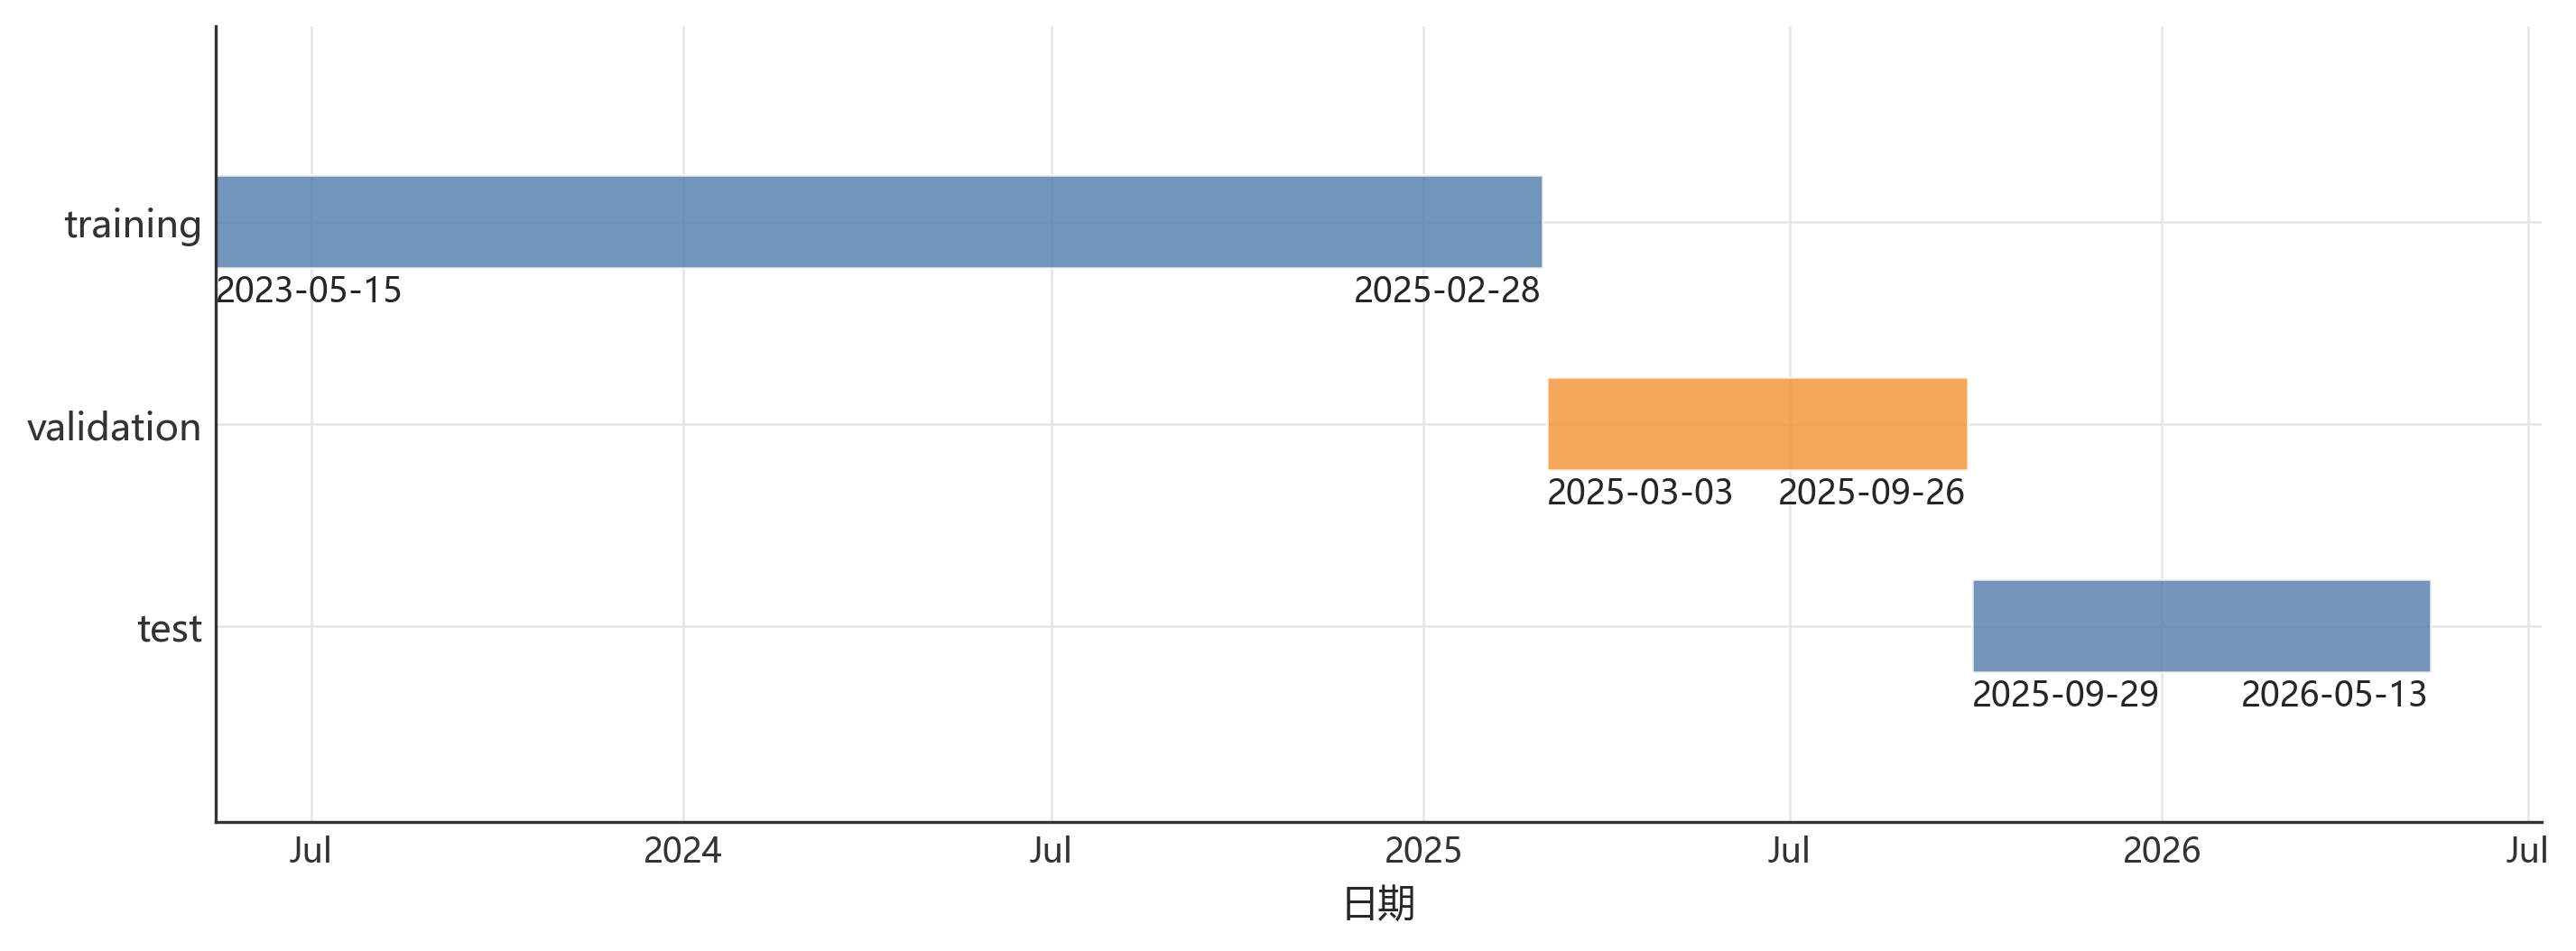
\includegraphics[width=0.90\textwidth]{figures/fig_timeline.png}
    \caption{训练、验证与测试样本划分。图中按照时间顺序展示本文样本外检验的三个区间，其中训练期用于标准化参数、标签阈值和模型参数估计，验证期用于模型选择，测试期仅用于最终样本外评价。}
    \label{fig:timeline}
\end{figure}

\subsection{核心变量定义}

本文核心变量围绕短时压力代理指标、未来压力标签和市场共同状态展开。所有需要标准化的变量均使用训练期历史信息，且以股票-日内 slot 为单位计算基准位置和尺度，避免同日未来信息或全样本信息进入特征。

\begin{table}[tbp]
\centering
\caption{核心变量、压力标签与防泄漏边界}
\label{tab:variables}
\small
\begin{threeparttable}
\begin{tabularx}{\textwidth}{p{0.18\textwidth}p{0.24\textwidth}Y}
\toprule
变量 & 含义 & 构造与解释边界 \\
\midrule
LSI(k) & 个股短时压力指数 & 由 ILLIQ、Range、RV 与 RelAmt 训练期股票-日内 slot 标准化后合成；属于压力代理指标。 \\
MarketLSI & 市场压力指数 & 个股 LSI 的市场层面聚合；仅使用当前及历史分钟信息。 \\
Stress\_H5 & 未来 5 分钟压力标签 & 未来窗口压力是否超过训练期阈值；只作为目标变量。 \\
Stress\_H10 & 未来 10 分钟压力标签 & 未来窗口压力是否超过训练期阈值；只作为目标变量。 \\
IndexRet & 市场收益状态 & 分钟收益的市场聚合，用于 QVAR 和预警特征。 \\
IndexRV & 市场波动状态 & 分钟收益平方的市场聚合，用于 QVAR 和预警特征。 \\
MarketRelAmt & 市场成交承接力 & 成交额相对历史基准的市场聚合；数值越低表示成交收缩。 \\
\bottomrule
\end{tabularx}
\begin{tablenotes}[flushleft]
\footnotesize
\item 注：CrossStress 只在 QVAR 中作为截面压力状态变量，不进入最终 SMARTBoost 特征矩阵。
\end{tablenotes}
\end{threeparttable}
\end{table}


表 \ref{tab:variables} 汇总了后续章节使用的主要变量。在特征边界核查中，CrossStress 被识别为由未来压力标签聚合得到的变量，故未纳入最终预测特征矩阵。

\subsection{样本覆盖与数据质量}

在进入模型估计前，需要确认分钟面板在证券和时间维度上具有足够稳定的覆盖。图 \ref{fig:coverage} 按股票和月份汇总有效分钟覆盖率，用于检查样本是否存在系统性缺口。

\begin{figure}[tbp]
    \centering
    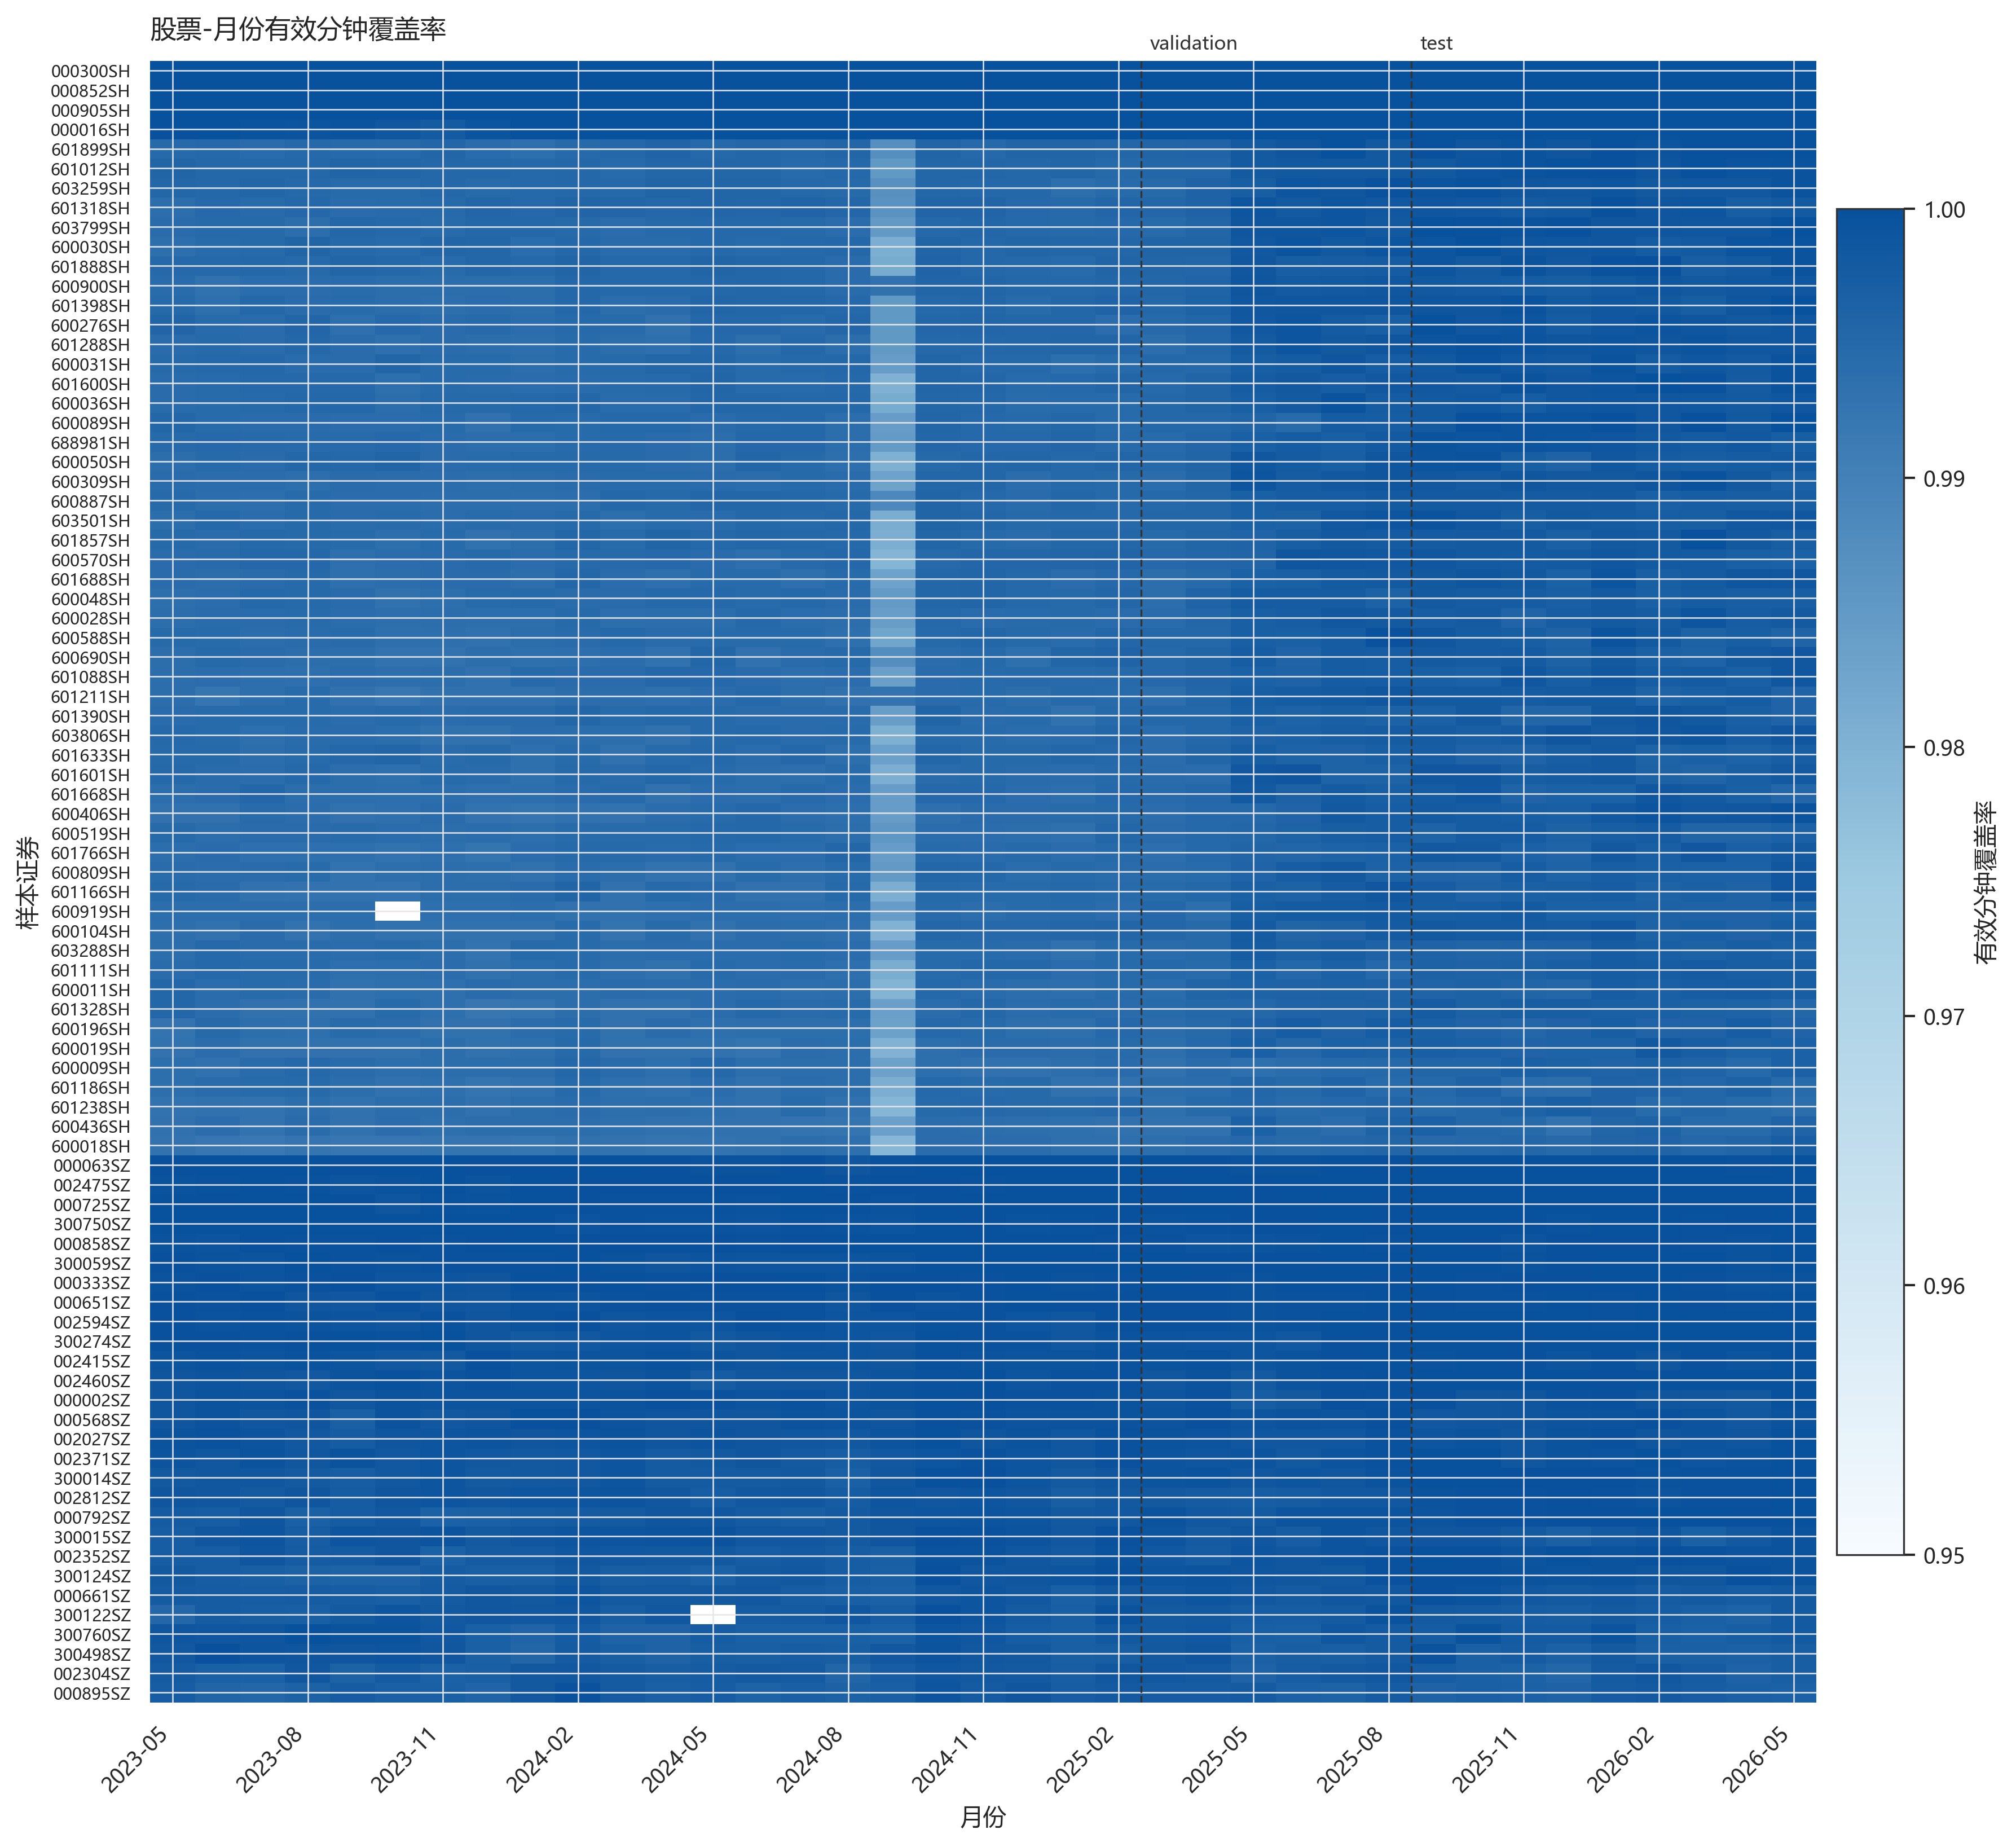
\includegraphics[width=0.90\textwidth]{figures/fig_coverage.png}
    \caption{股票-月份有效分钟覆盖率热力图。颜色表示对应股票在对应月份的有效分钟覆盖程度，用于检验分钟面板在横截面和时间维度上的连续性。}
    \label{fig:coverage}
\end{figure}

图 \ref{fig:coverage} 表明，样本在多数股票和月份上具有较稳定的有效分钟覆盖，未呈现集中于单一时期或单一证券的系统性缺口。因此，后续描述性事实、动态风险度量和样本外预警检验可以建立在相对完整的高频面板之上。

热力图的核心作用在于验证分钟面板是否存在集中性缺口，而非证明数据完全无遗漏。图中个别浅色区域对应特定证券在局部月份的有效分钟覆盖下降，可能源于阶段性停牌或数据报送差异，属于局部现象，不构成跨时期的系统性样本偏误。训练、验证与测试三个区间的整体覆盖水平较为接近，有助于排除样本外检验结论由测试期数据缺失驱动的可能性。

\subsection{LSI 日内模式}

高频压力指标具有明显日内结构。为观察短时压力是否具有稳定的日内结构，图 \ref{fig:intraday} 展示了 \(\LSI_{5}\) 在不同日内 slot 上的均值、中位数和分位带。

\begin{figure}[tbp]
    \centering
    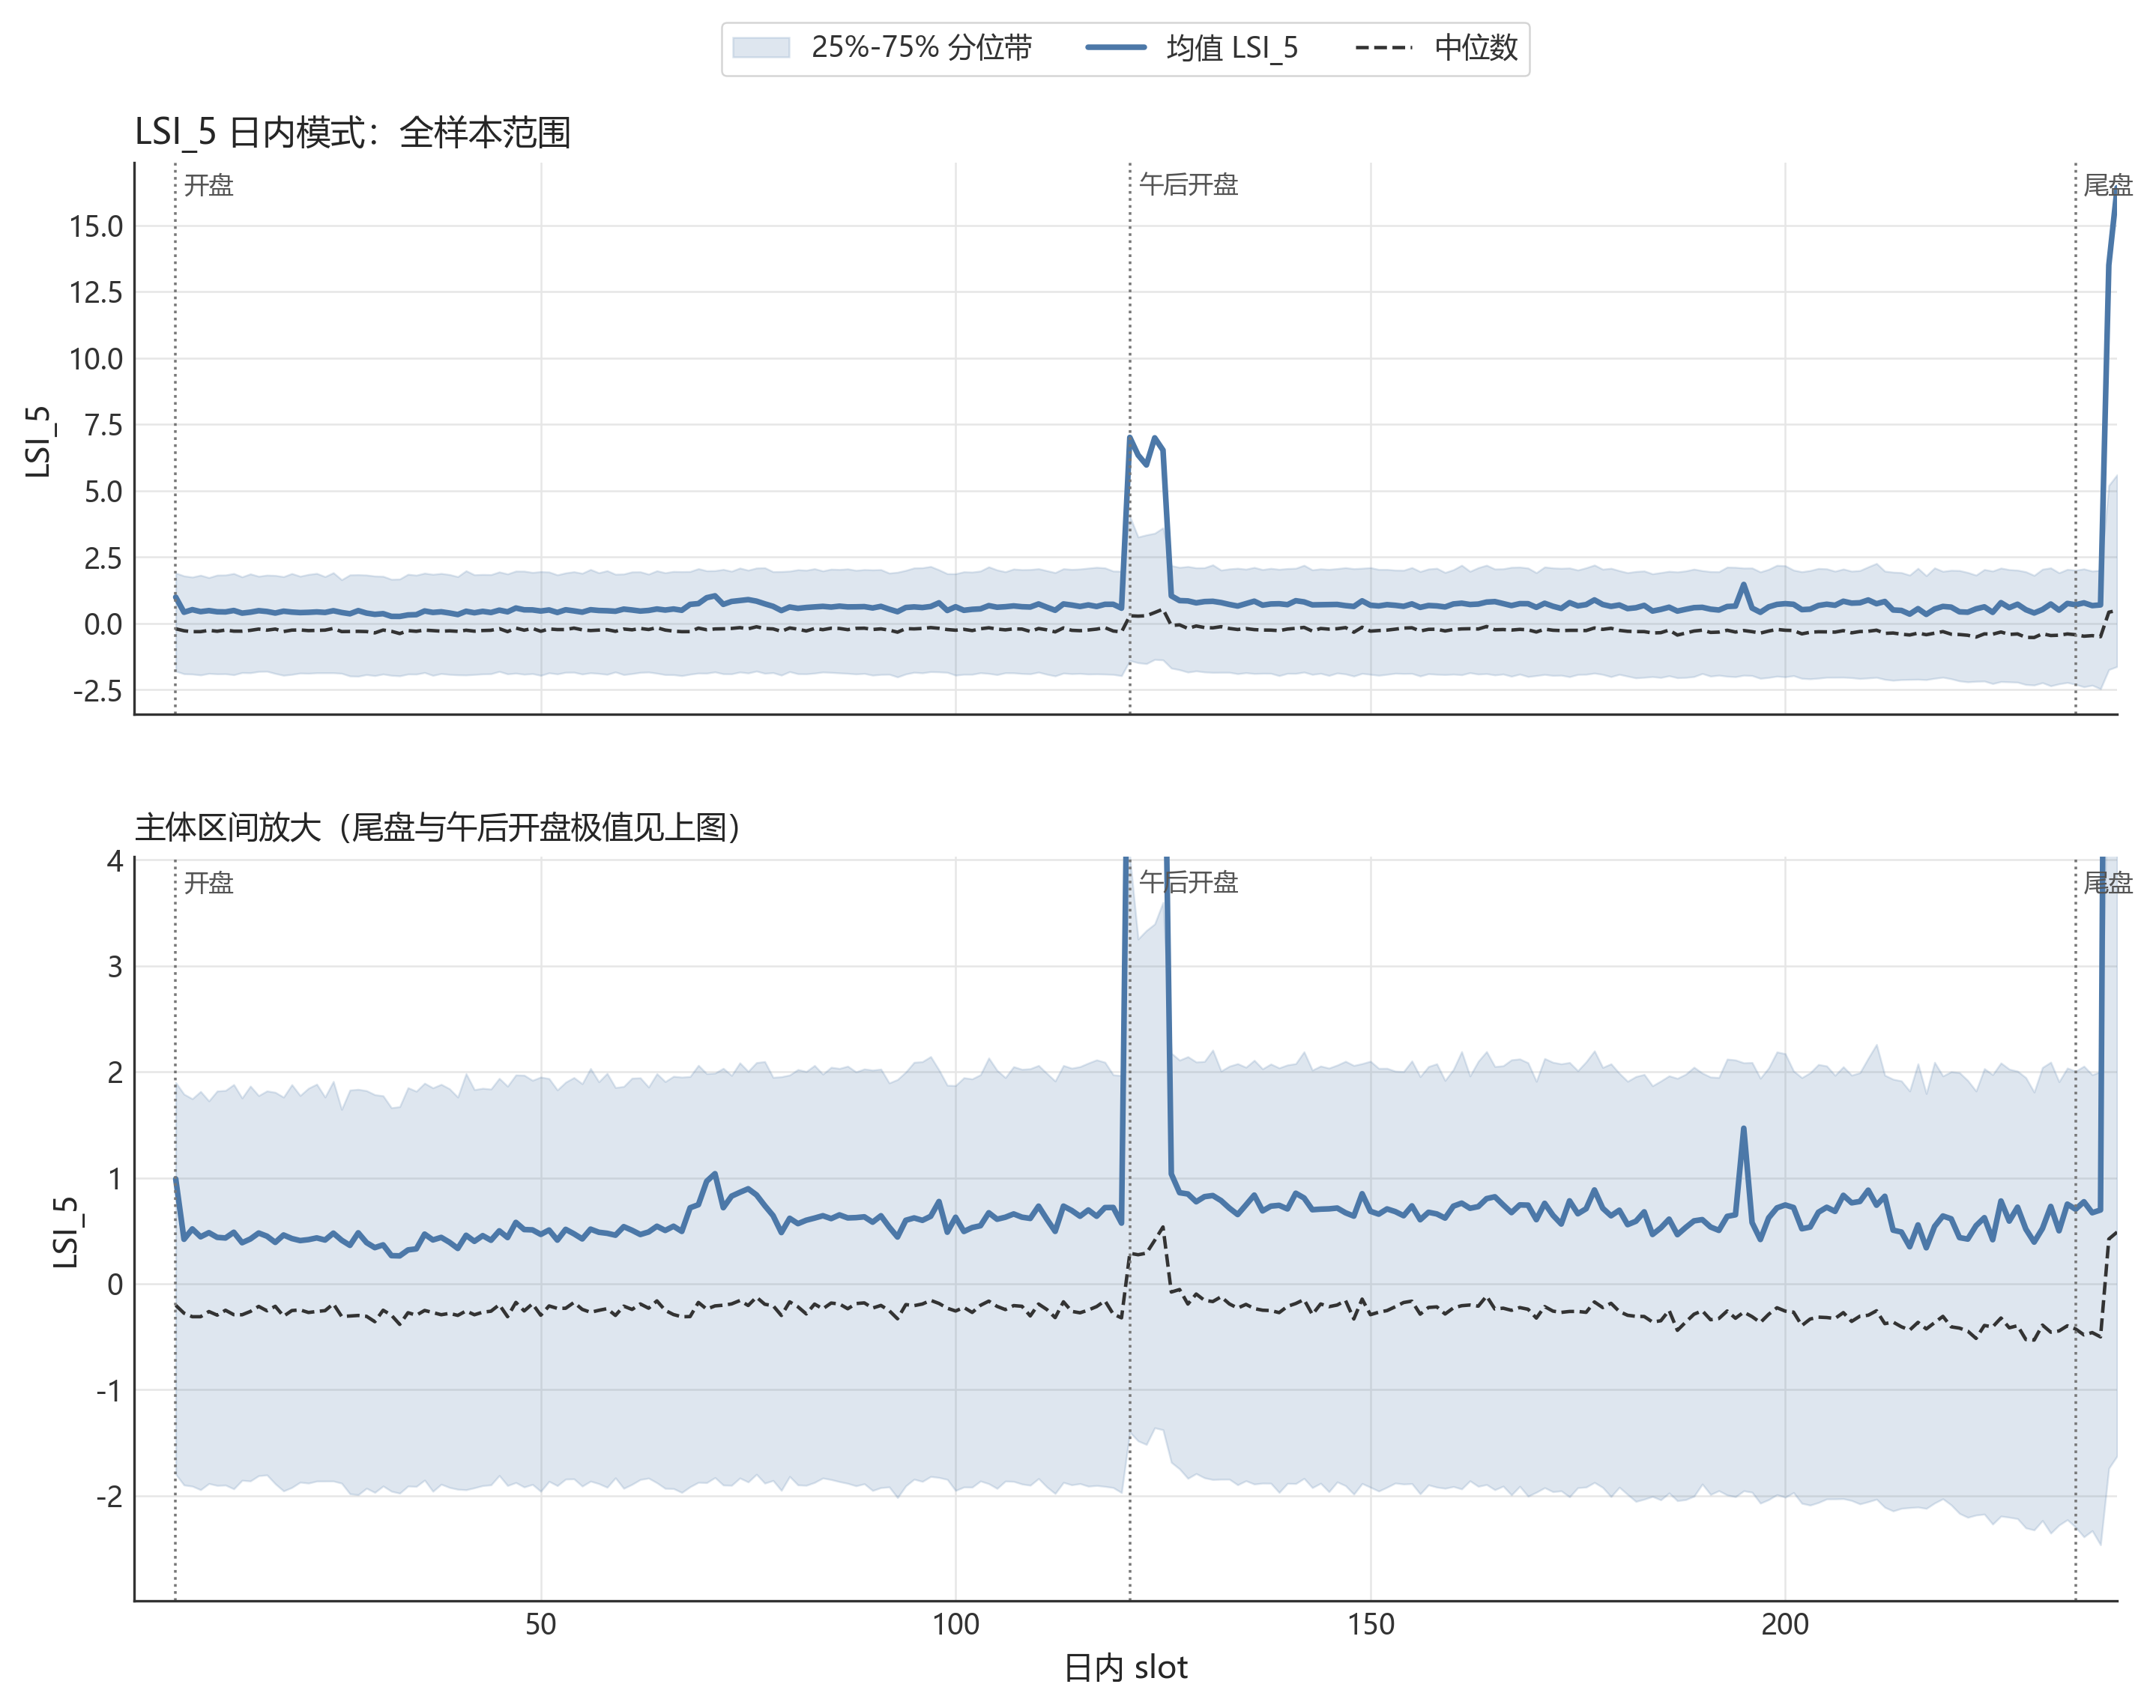
\includegraphics[width=0.90\textwidth]{figures/fig_intraday.png}
    \caption{LSI\_5 日内模式。图中保留 LSI 术语，并使用分位带展示横截面与日期维度下的离散程度。}
    \label{fig:intraday}
\end{figure}

可以看到，LSI 在开盘、午后开盘和尾盘附近更容易出现局部抬升，说明短时压力并非均匀分布于全天。这也解释了本文为什么采用股票—日内 slot 的训练期稳健标准化。

高频流动性压力的日内节奏意味着，若不加以控制地跨时间片比较样本，可能将开盘或尾盘附近的正常交易节律误判为异常压力抬升。本文在股票—日内时间片层面使用训练期历史分布确定标准化参数，目的是使后续特征和标签尽量反映相对于正常节律的偏离程度，而非吸收时间片本身的固定效应。

\subsection{MarketLSI 与压力事件率}

市场层面的压力动态也具有时变性。图 \ref{fig:marketlsi} 将 MarketLSI 按日聚合，并叠加滚动趋势和样本区间背景。

\begin{figure}[tbp]
    \centering
    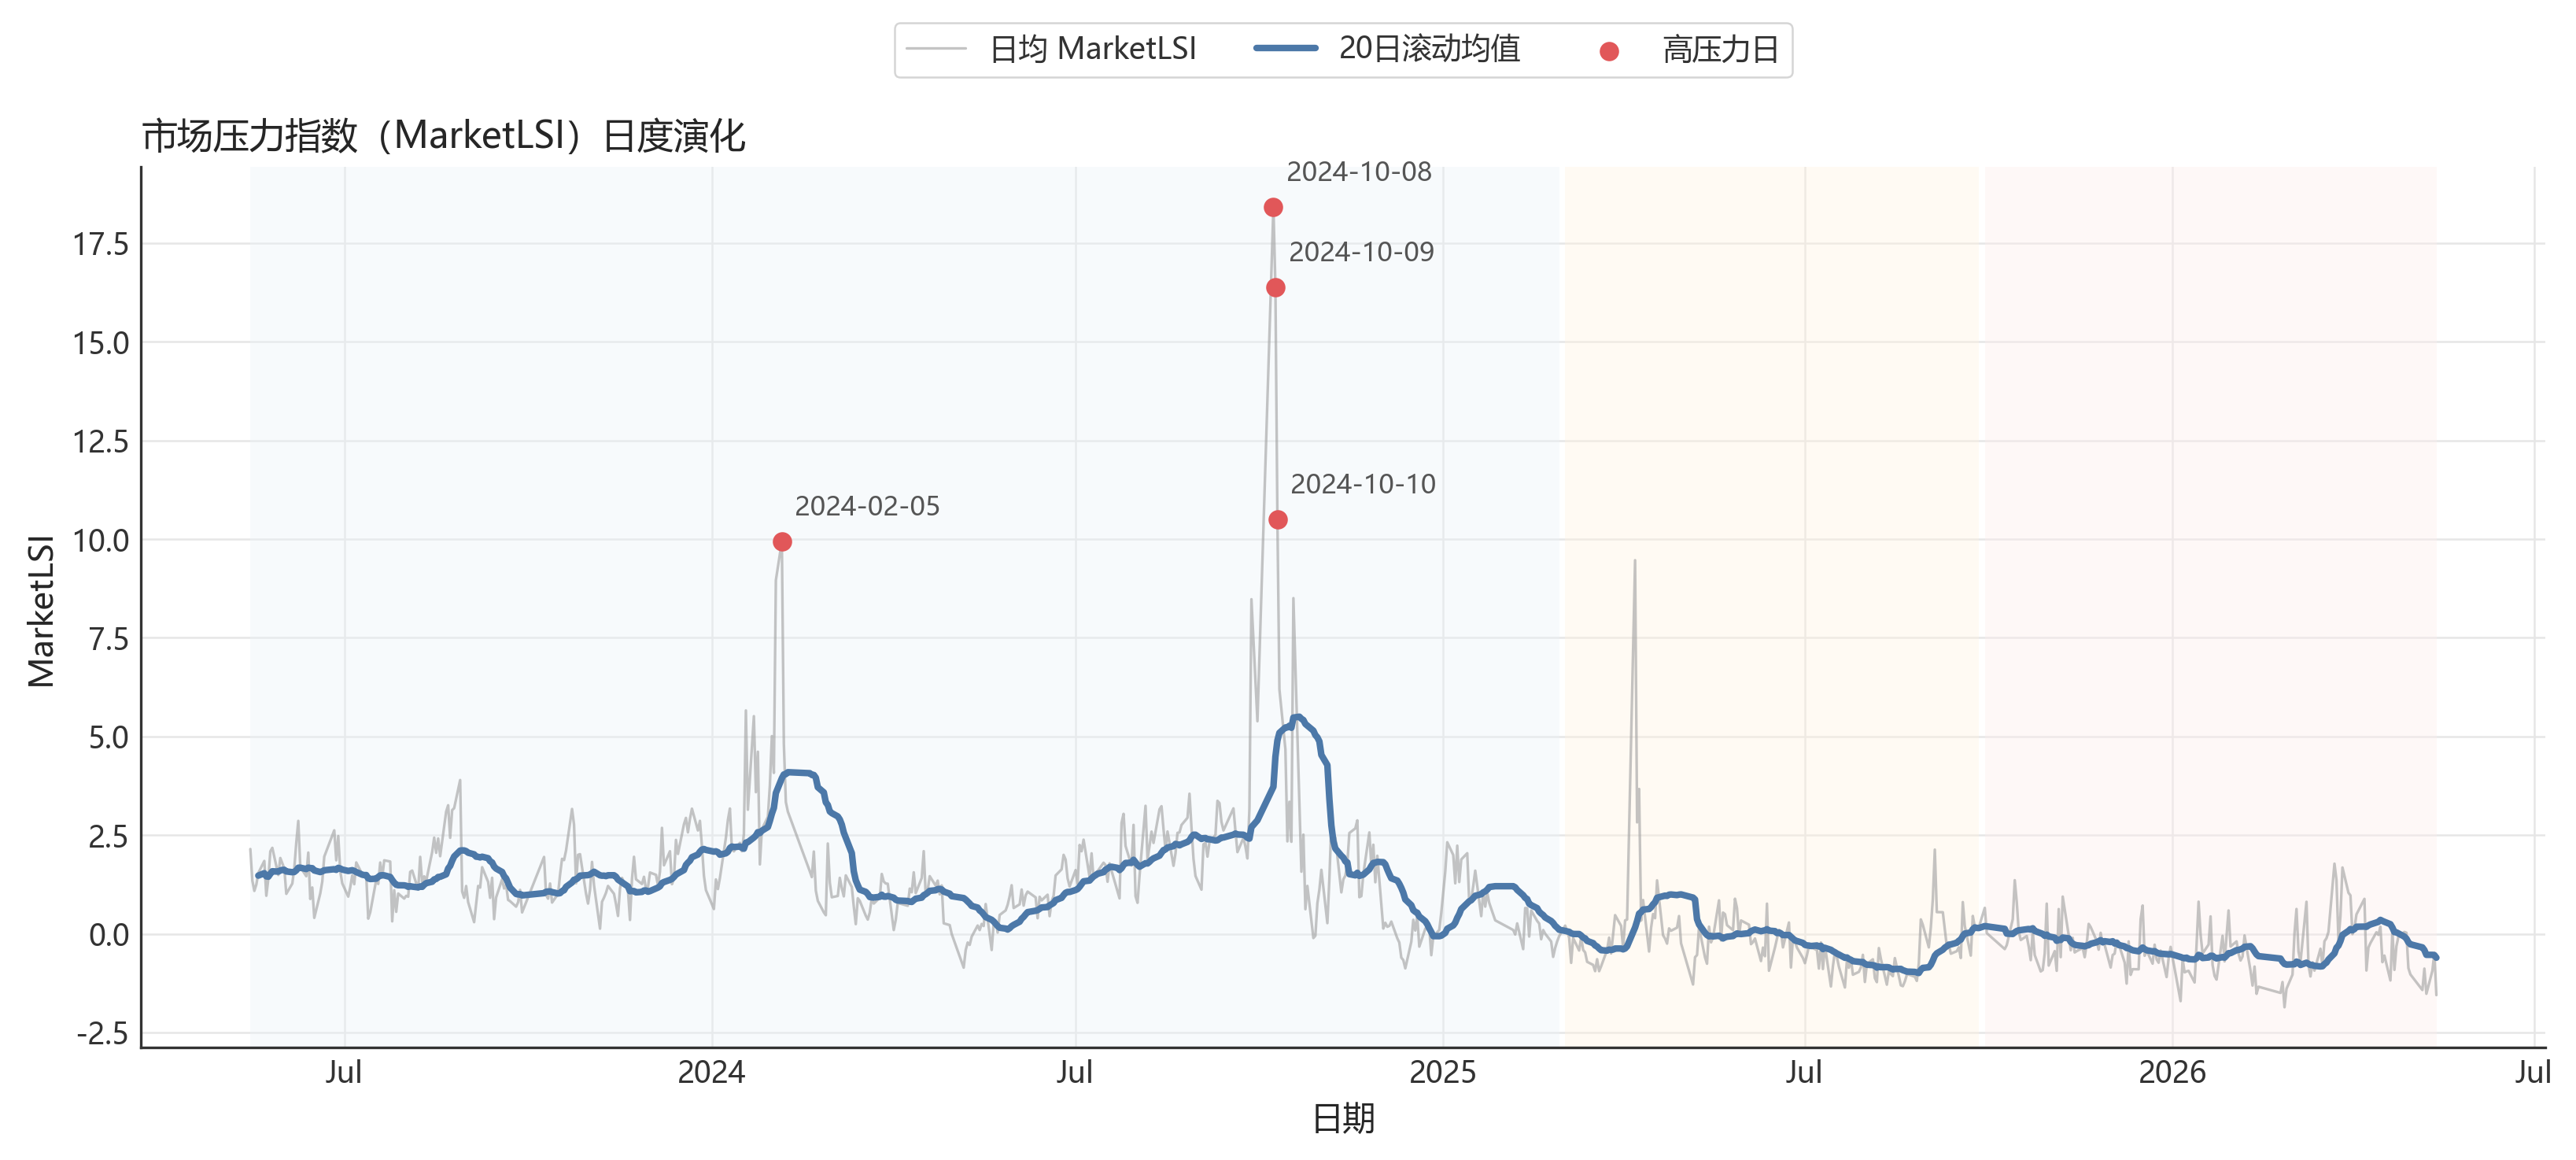
\includegraphics[width=0.94\textwidth]{figures/fig_marketlsi.png}
    \caption{市场压力指数（MarketLSI）日度时间序列。背景区间对应训练、验证与测试样本划分，峰值标记用于辅助识别高压力时段。}
    \label{fig:marketlsi}
\end{figure}

该图显示市场压力存在阶段性抬升和局部峰值，但这些阶段背景只用于描述时间异质性，不构成因果识别。

MarketLSI 作为截面层面共同压力的描述性代理指标，捕捉的是横截面内多数证券同步出现压力抬升的整体背景，而非个别证券行为或外生冲击的因果特征。由此引出后文评价指标的选择依据：鉴于测试期压力事件更为稀有，整体分类准确率因大量非事件样本而趋于虚高，难以有效衡量稀有事件的排序能力，因此本文优先报告 PR-AUC、Top 5\% 命中率和 lift。

\begin{table}[tbp]
\centering
\caption{未来压力标签的样本区间分布}
\label{tab:label-distribution}
\small
\begin{threeparttable}
\begin{tabular}{lcc}
\toprule
样本区间 & Stress\_H5 事件率 & Stress\_H10 事件率 \\
\midrule
train & 10.05\% & 10.06\% \\
validation & 5.05\% & 5.27\% \\
test & 5.44\% & 5.80\% \\
\bottomrule
\end{tabular}
\begin{tablenotes}[flushleft]
\footnotesize
\item 注：事件率按样本区间汇总；标签阈值只由训练期历史分布确定。
\end{tablenotes}
\end{threeparttable}
\end{table}


表 \ref{tab:label-distribution} 显示，训练期标签阈值约束下的事件率接近 10\%，而验证期和测试期事件率更低。这说明样本外预警任务具有高度不平衡性，因此后文在 SMARTBoost 评价中优先使用 PR-AUC、Top 5\% 命中率和 lift，而不把 ROC-AUC 作为唯一依据。

\FloatBarrier
